\documentclass{article}

% Import packages
\usepackage{amsmath}
\usepackage{listings}
\usepackage{graphicx}
\usepackage{float}
\usepackage{color}
\usepackage{booktabs}
\usepackage{caption}
\usepackage{hyperref}
\usepackage{placeins}

% Tweak vertical caption spacing
\captionsetup[table]{skip=10pt}

% Custom commands
\newcommand{\lrp}[1]{\left(#1\right)}
\newcommand{\lrb}[1]{\left[#1\right]}

% Setup listing properties
\definecolor{mygray}{rgb}{0.5,0.5,0.5}
\lstset{language=fortran}
\lstset{backgroundcolor=\color{white}}
\lstset{frame=none}
\lstset{numbers=none}
\lstset{numbersep=10pt}
\lstset{numberstyle=\color{mygray}}
\lstset{basicstyle=\ttfamily, basewidth=0.5em}
\lstset{stringstyle=\ttfamily}
%\lstset{keywordstyle=\color{red}\bfseries}
\lstset{commentstyle=\itshape\color{blue}}
\lstset{showspaces=false}
\lstset{showstringspaces=false}
\lstset{showtabs=false}
\lstset{breaklines=true}
\lstset{aboveskip=20pt,belowskip=20pt}
\lstset{moredelim=**[is][\color{blue}]{@}{@}}

\begin{document}

% Title
\title{\bfseries FYS4150 Project 2}
\author{Alex Ho\\Lars Frogner}
\date{\today}
\pagenumbering{gobble}
\maketitle

\begin{abstract}
	We study a simple case of the quantum mechanical system consisting of one or two electrons in a three-dimensional harmonic oscillator potential. The governing equation gives rise to an eigenvalue problem, which we solve numerically using the Jacobi eigenvalue method. 
\end{abstract}

% Table of contents
\tableofcontents
\newpage
\pagenumbering{arabic}

\section{Introduction}
In this project, we will have a look at the so called \textit{Eigenvalue problem}. We will use the well known Schroedinger equation from quantum mechanics and apply it to a system consisting of a single electron in a harmonic oscillator (HO) potential. To achieve this, we will implement Jacobi's method to solve the Schroedinger equation and then find the eigenvalues, which will physically be the energies of the electrons. We will also look at the case where we have two electrons in a three dimensional harmonic oscillator, and study the system for different potential strengths with and without interaction between the two electrons.\\\\
An overview of the physical problem is given in section \ref{section:prob}, followed by a derivation of the algorithm for solving eigenvalue problems with Jacobi's method in section \ref{section:alg}. For this report we have used two independent implementations of the algorithm; one in C++ and one in Fortran 2008. The respective source codes can be found in the following GitHub repositories:\\\\
C++:\\\url{https://github.com/AHo94/FYS3150_Projects/tree/master/Project2}\\\\
Fortran:\\\url{https://github.com/lars-frogner/FYS4150-Projects/tree/master/Project%202}\\\\
Section \ref{section:unit} describes the unit tests that were used to verify that the code worked correctly. The results for the two physical problems are presented in sections \ref{section:onee} and \ref{section:twoe} respectively, while section \ref{section:iters} evaluates the number of iterations used by the algorithm. Finally, we summarise our findings in section \ref{section:conc}.

\section{Methods}
\subsection{Electrons in HO potential} \label{section:prob}
The Schroedinger equation for the radial component of the wave function $R$ of the an electron in a spherically symmetric potential $V(r)$ is
\begin{align}
	-\frac{\hbar^2}{2m}\lrp{\frac{1}{r^2}\frac{d}{dr}\lrp{r^2\frac{d}{dr}} - \frac{l(l+1)}{r^2}}R(r) + V(r)R(r) = ER(r) \label{eq:schr}
\end{align}
where $m$ is the mass of the electron, $l=0,1,2,\ldots$ is the orbital momentum quantum number and $E$ is the energy of the system. For a harmonic oscillator potential we have 
\begin{align*}
	V(r) = \frac{1}{2}m\omega^2r^2
\end{align*}
where $\omega$ is the angular frequency. The associated energies are then
\begin{align*}
	E_{nl} = \hbar\omega\lrp{2n + l + \frac{3}{2}},
\end{align*}
where $n = 0, 1, 2, \ldots$ is the energy quantum number. For this potential, and with no angular momentum ($l = 0$), we can write \ref{eq:schr} in the following dimensionless form:
\begin{align*}
	-\frac{d^2}{d\rho^2}u(\rho) + \rho^2u(\rho) = \lambda_n u(\rho)
\end{align*}
Here $u \equiv rR$, $\rho \equiv r/\alpha$ and $\lambda_n \equiv 2m\alpha^2E_{n0}/\hbar^2$, where $\alpha = (\hbar^2/mk)^{1/4}$. The $\rho^2$ factor is just the potential, $V(\rho) = \rho^2$. The boundary conditions are $u(\rho = 0) = u(\rho = \infty) = 0$. Defining a grid of $N+2$ points $\rho_0, \rho_1, \ldots, \rho_{N+1}$ separated by $h = (\rho_{N+1} - \rho_0)/(N+1)$, and approximating the second derivative with a simple three-point formula yields the following discretised equation:
\begin{align*}
	-\frac{u_{i+1} - 2u_i + u_{i-1}}{h^2} + V_iu_i = \lambda_n u_i, \qquad i = 1, \ldots, N
\end{align*}
The boundary conditions are now $u_0 = u(\rho_0) = u(0) = 0$ and $u_{N+1} = u(\rho_{N+1}) = u(\rho_\text{max}) = 0$, where the value for $\rho_\text{max}$ must be chosen large enough so that the solution can go naturally to zero without being forced by the artificial boundary condition. Writing the above equation in matrix form gives us the final form of the eigenvalue problem:
\begin{align} \label{eq:matreq}
	\lrp{\begin{array}{ccc}
		2h^{-2} + V_1 & -h^{-2} & 0 \\
		-h^{-2} & 2h^{-2} + V_2 & -h^{-2} \\
		\vdots & \vdots & \vdots \\
		0 & -h^{-2} & 2h^{-2} + V_N
	\end{array}}
	\lrp{\begin{array}{c}
	u_1 \\
	u_2 \\
	\vdots \\
	u_N
	\end{array}} = \lambda_n
	\lrp{\begin{array}{c}
	u_1 \\
	u_2 \\
	\vdots \\
	u_N
	\end{array}}
\end{align}
So the coefficient matrix is tridiagonal, with $2h^{-2} + V_i$ on the main diagonal and $-h^{-2}$ on the upper and lower diagonal. The boundary values are left out since they are known to be zero. This problem will be solved numerically with the Jacobi eigenvalue method.\\\\
A simple two-body variant of this problem can be studied without any other modifications than changing the potential. The Schroedinger equation for the interacting two-electron wave function can be formulated in terms of the position of the centre of mass and the separation of the electrons. Assuming that the centre of mass stays put at the origin (and still assuming no angluar momentum), the dimensionless equation for the wave function can be written as
\begin{align*}
	-\frac{d^2}{d\rho^2}u(\rho) + \lrp{\omega_r^2\rho^2 + \frac{1}{\rho}}u(\rho) = \lambda_n u(\rho)
\end{align*}
where $\rho$ is now the separation of the particles (which is twice the distance from the origin, which in turn is the same for both particles since the centre of mass is at the origin), in units of the length scale $\alpha$ which is now defined as $\alpha = \hbar^2/m\beta e^2$. Here $\beta$ is Coloumb's constant and $e$ is the electron charge. The strength of the HO potential is described by the parameter $\omega_r$. The $1/\rho$ term is the Coloumn potential describing the interaction between the electrons. The eigenvalues are related to the energy of the system by $\lambda_n = m\alpha^2E_{n0}/\hbar^2$. In order to solve this we can just use $V_i = \omega_r^2\rho_i^2$ (for the non-interacting case) or $V_i = \omega_r^2\rho_i^2 + 1/\rho_i$ (for the interacting case) in \eqref{eq:matreq}.

\subsection{The Jacobi eigenvalue method} \label{section:alg}
The Jacobi eigenvalue method involves reducing a symmetric matrix into a diagonal matrix with the same eigenvalues. This is achieved by applying a series of strategically chosen similarity transformations that eliminate off-diagonal elements one by one. A similarity transformation preserves the eigenvalues. To see this, consider a symmetric matrix $A$ with an eigenvalue $\lambda$ and eigenvector $\mathbf{v}$:
\begin{align*}
	A\mathbf{v} = \lambda\mathbf{v}
\end{align*}
We multiply both sides from the left with the transpose of an orthogonal matrix $S$, and also insert $I = SS^T$ between $A$ and $\mathbf{v}$ on the left hand side:
\begin{align*}
	S^TASS^T\mathbf{v} = \lambda S^T\mathbf{v}
\end{align*}
So the similarity transformation yields a matrix $A' = S^TAS$ which has the same eigenvalue $\lambda$. The corresponding eigenvector is $S^T\mathbf{v}$.\\\\
For the Jacobi method we use a transformation matrix on the following form:
\begin{align*}
	S = \left(\begin{array}{ccccccc}
		1 &&&&&& 0 \\
		& \ddots &&&&& \\
		&& \cos{\theta} & \cdots & \sin{\theta} && \\
		&& \vdots & 1 & \vdots && \\
		&& -\sin{\theta} & \cdots & \cos{\theta} && \\
		&&&&& \ddots & \\
		0 &&&&&& 1 \\
	\end{array}\right)
\end{align*}
It has the same structure as the identity matrix, except that the 2x2 sub-matrix formed by the four intersections of columns and rows $k$ and $l$ is a rotation matrix. So $S$ performs a rotation of angle $\theta$ in the $(k, l)$-plane. The idea behind the algorithm is that for each iteration, $\theta$ can be chosen such that the element $a_{kl} = a_{lk}$ becomes zero. To see how we can do this, we first write out the results of a similarity transformation $A' = {S}^TAS$ with $S$:
\begin{align}
	a'_{ik} &= ca_{ik} - sa_{il} \qquad (i \neq k,\:i \neq l) \label{eq:tr1} \\
	a'_{il} &= ca_{il} + sa_{ik} \qquad (i \neq k,\:i \neq l) \label{eq:tr2} \\
	a'_{kk} &= c^2a_{kk} + s^2a_{ll} - 2sca_{kl} \\
	a'_{ll} &= s^2a_{kk} + c^2a_{ll} + 2sca_{kl} \label{eq:tr4} \\
	a'_{kl} &= (c^2 - s^2)a_{kl} + sc(a_{kk} - a_{ll})
\end{align}
Here $c \equiv \cos{\theta}$ and $s \equiv \sin{\theta}$. All elements of $A$ that do not lie on rows or columns $k$ and $l$ are not affected by the similarity transformation. We want to find the angle that results in $a'_{kl} = 0$:
\begin{align*}
	(c^2 - s^2)a_{kl} + sc(a_{kk} - a_{ll}) = 0
\end{align*}
Dividing by $c^2$ gives
\begin{align*}
	&(1 - t^2)a_{kl} + t(a_{kk} - a_{ll}) = 0 \\
	\Rightarrow \quad &-a_{kl}t^2 + (a_{kk} - a_{ll})t + a_{kl} = 0
\end{align*}
where $t \equiv \tan{\theta}$. We then solve for $t$:
\begin{align*}
	t &= \frac{(a_{ll} - a_{kk}) \pm \sqrt{(a_{ll} - a_{kk})^2 + 4{a_{kl}}^2}}{2a_{kl}}
\end{align*}
Introducing the quantity
\begin{align}
	\tau = \frac{a_{ll} - a_{kk}}{2a_{kl}}, \label{eq:tau}
\end{align}
the expression for $t$ becomes
\begin{align*}
	t = \tau \pm \sqrt{1 + \tau^2}.
\end{align*}
We multiply with $\tau \mp \sqrt{1 + \tau^2}$ in the numerator and the denominator to get 
\begin{align}
	t = \frac{1}{-\tau \pm \sqrt{1 + \tau^2}}. \label{eq:tan}
\end{align}
There are two possible values for $t$ that can be used. The most stable approach is to choose the sign that gives the smallest absolute value, as this will result in the smallest possible rotation angle. Once we have $t$, we can then calculate the corresponding values for $c$ and $s$:
\begin{align}
	c &= \frac{1}{\sqrt{1 + t^2}} \label{eq:cos} \\
	s &= tc \label{eq:sin}
\end{align}
From equations \eqref{eq:tr1} and \eqref{eq:tr2} we can see that any off-diagonal elements that we have already eliminated can become non-zero again in the subsequent transformations. However, if we always choose to eliminate the (absolute) largest off-diagonal element in each iteration, we are still ensured that the matrix will become closer and closer to diagonal (see \cite{cpyhsics} for proof).\\\\
Once we have the matrix on diagonal form $D$, the eigenvalues are just the diagonal elements. The eigenvectors are the columns of the matrix $R = S_1S_2\ldots S_n$ (the product of all the transformation matrices $S$), since we have
\begin{align*}
	&R^TAR = D \\
	\Rightarrow \quad &A = RDR^T \\
	\Rightarrow \quad &AR = RD
\end{align*}
which we can write in terms of the columns $\mathbf{r}_i$ of $R$ as
\begin{align*}
	A\mathbf{r}_i = \lambda_i\mathbf{r}_i.
\end{align*}
So in order to obtain the eigenvectors, we start with $R$ equal to the identity matrix, and for each iteration update the eigenvectors by computing
\begin{align*}
	R' = RS.
\end{align*}
From this the new elements become
\begin{align}
	r'_{ik} = cr_{ik} - sr_{il} \label{eq:etr1} \\
	r'_{il} = sr_{ik} + cr_{il} \label{eq:etr2}
\end{align}
while the remaining elements don't change.\\\\
Let us summarise the algorithm. For each iteration, we perform the following steps:
\begin{enumerate}
	\item Find the largest off-diagonal element and its position $(k, l)$.
	\item If it is smaller than some tolerance, we consider the matrix to be diagonal and stop iterating.
	\item Otherwise, use \eqref{eq:tau}, \eqref{eq:tan}, \eqref{eq:cos} and \eqref{eq:sin} to calculate $s$ and $c$.
	\item Update the required matrix elements using \eqref{eq:tr1} through \eqref{eq:tr4}. The $a'_{kl} = a'_{lk}$ element is just set explicitly to zero.
	\item Update the eigenvectors using \eqref{eq:etr1} and \eqref{eq:etr2}.
\end{enumerate}

\subsection{Unit testing} \label{section:unit}
Several properties of a matrix will be conserved during a similarity transformation. In order to make sure that we implemented the transformations correctly, we wrote code for displaying some of these properties so that we could check that they indeed didn't change from iteration to iteration.\\\\
For instance, a symmetric matrix should remain symmetric after a similarity transformation, so the Fortran program has the option to print the matrix for inspection in each iteration. Displaying the maximum off-diagonal element as well allowed us to make sure that the correct elements were being selected for elimination. To check this in the C++ program, a test matrix is constructed with equal off-diagonal elements except for one value which is set to -1000. If this element is not selected as the largest off-diagonal element, then we know that something is wrong with the implementation. \\\\
In addition, the Frobenius norm,
\begin{align*}
	\lVert A\rVert_F = \sqrt{\sum_{i=1}^n\sum_{j=1}^n|a_{ij}|^2},
\end{align*}
must also be conserved. So a simple unit test is to print the Frobenius norm in each iteration to reveal whether or not it changes.\\\\
Finally, we can use the fact that orthogonality is preserved for an orthogonal and/or unitary vector transformation. To show this, let us consider the following basis of vectors
\begin{align}
\mathbf{v}_i = \begin{pmatrix}
v_{i1} \\
v_{i2} \\
\vdots \\
v_{in}
\end{pmatrix}
\end{align}
We will also assume that this is an orthogonal basis
\begin{align}
\mathbf{v}_j^T\mathbf{v}_i = \delta_{ij}
\end{align}
We want to look at the orthogonality properties for a orthogonal and unitary vector transformation in the form
\begin{align}
\mathbf{w}_i = \mathbf{U}\mathbf{v}_i
\end{align}
For an orthogonal matrix, we know that $\mathbf{U}^T\mathbf{U} = \mathbf{I}=1$, where $\mathbf{I}$ is the identity matrix, so we have that
\begin{align}
\mathbf{w}_j^T\mathbf{w}_i = (\mathbf{U}\mathbf{v}_i)^T(\mathbf{U}\mathbf{v}_i) = \mathbf{v}_j^T \mathbf{U}^T\mathbf{U}\mathbf{v}_i = \mathbf{v}_i^T\mathbf{v}_i = \delta{ij}
\end{align}
For a unitary matrix, we have that $\mathbf{U^*}\mathbf{U}=\mathbf{I}$ and $\mathbf{U}^{\dagger}\mathbf{U} = \mathbf{I}$, where $\mathbf{U}^{\dagger} = (\mathbf{U}^*)^T$ is the hermitian conjugate. Doing the hermitian conjugate on the transformation vector, we can show that
\begin{align}
\mathbf{w}_j^{\dagger}\mathbf{w}_i = (\mathbf{U}\mathbf{v}_j)^{\dagger}(\mathbf{U}\mathbf{v}_i) = \mathbf{v}_j^{\dagger}\mathbf{U}^{\dagger}\mathbf{U}\mathbf{v}_i = \mathbf{v}_j^{\dagger}\mathbf{v}_i = \delta_{ij}
\end{align}
Here we have assumed that the basis vector is real, so $\mathbf{v}_i^* = \mathbf{v}_i$.\\\\
The Jacobi method uses an orthogonal transformation, so one can expect that the resulting eigenvectors remain orthogonal. We have therefore implemented units test that print the inner products of the different eigenvectors with each other. Since the vectors must be orthogonal to each other, these values should always be zero.

\section{Results}
\subsection{Single electron} \label{section:onee}
In the C++ program, by selecting the number of mesh points to $n=400$, with $\rho_{max} = 10$, the output for the non interacting case is the following:
\begin{lstlisting}
@
Using a 400x400 matrix (n = 400)
with rho_max = 10

Max (absolute) value in the test matrix: 1000
max_diag does give out the largest value
max_diag result: 1000 

Starting Jacobi's algorithm for a single electron
Time elapsed for non interactive case: 400.941s
Number of iterations: 260506
Lowest 3 eigenvalues are: 
2.99981
6.99903
10.9976
Possible number of orthogonal vectors: 79800
Number of orthogonal vectors: 79800
Number of non-orthogonal vectors: 0

Using Armadillo to compare the time

Lowest 3 eigenvalues of the Armadillo simulation: 
2.99981
6.99903
10.9976
Time elapsed for Armadillo's algorithm: 0.347s
\end{lstlisting}
The eigenvalues, even though they are not within 4 decimal precision, are very close to the exact analytical eigenvalues. We can also see that the number of iterations needed to fully diagonalize the matrix $\mathbf{A}$ (or at least within a tolerance $\epsilon$) was 260506 iterations. The unit test of the orthogonality between the eigenvectors is also shown, where every possibly combination of the scalar product between the eigenvectors are orthogonal (also within a tolerance).\\\\
The time it took for the program to run was roughly 6 minutes. This seems like a very long simulation time, so there is probably something that is not quite optimal in the program, thus causing the program to run for a longer time. Compared to Armadillo's \emph{eig\_sym}, we can clearly see that Armadillo is much faster, using less than a second to finish. The lowest three eigenvalues are identical to our Jacobi's method, so Armadillo's method can serve as a good unit test for the eigenvalues.\\\\
The output from the Fortran program is represented in table \ref{table:selprob300}, which shows the first three eigenvalues for 300 grid points and $\rho_\text{max} = 5$.\\
\begin{table}[!h]
	\caption{Single-electron eigenvalues ($n$ = 300, $\rho_{max}$ = 5)}
	\centering
	\begin{tabular}{l}
		\toprule
		$\lambda$ \\ [0.5ex]
		\midrule
		2.9999 \\
		6.9996 \\
		10.9991 \\
		\bottomrule
	\end{tabular}
	\label{table:selprob300}
\end{table}\\
We see that they agree with the analytical values 3, 7 and 11 down to the third decimal place. Fewer grid points than 300 only gave agreement down to the second decimal place. $\rho_\text{max} = 5$ seems to be a good compromise between having infinity at a large enough distance and getting good enough resolution for small $\rho$ (which is where the interesting things happen).\\\\
The C++ and Fortran implementations apparently agree quite well about the eigenvalues. This is indeed the case for all the results, so we will no longer distinguish between results from the two implementations. \\\\
The probability distributions (the eigenvectors squared) for the three lowest energy states are shown in figure \ref{fig:selprob300}.\\
\begin{figure}[!h]
	\centering
	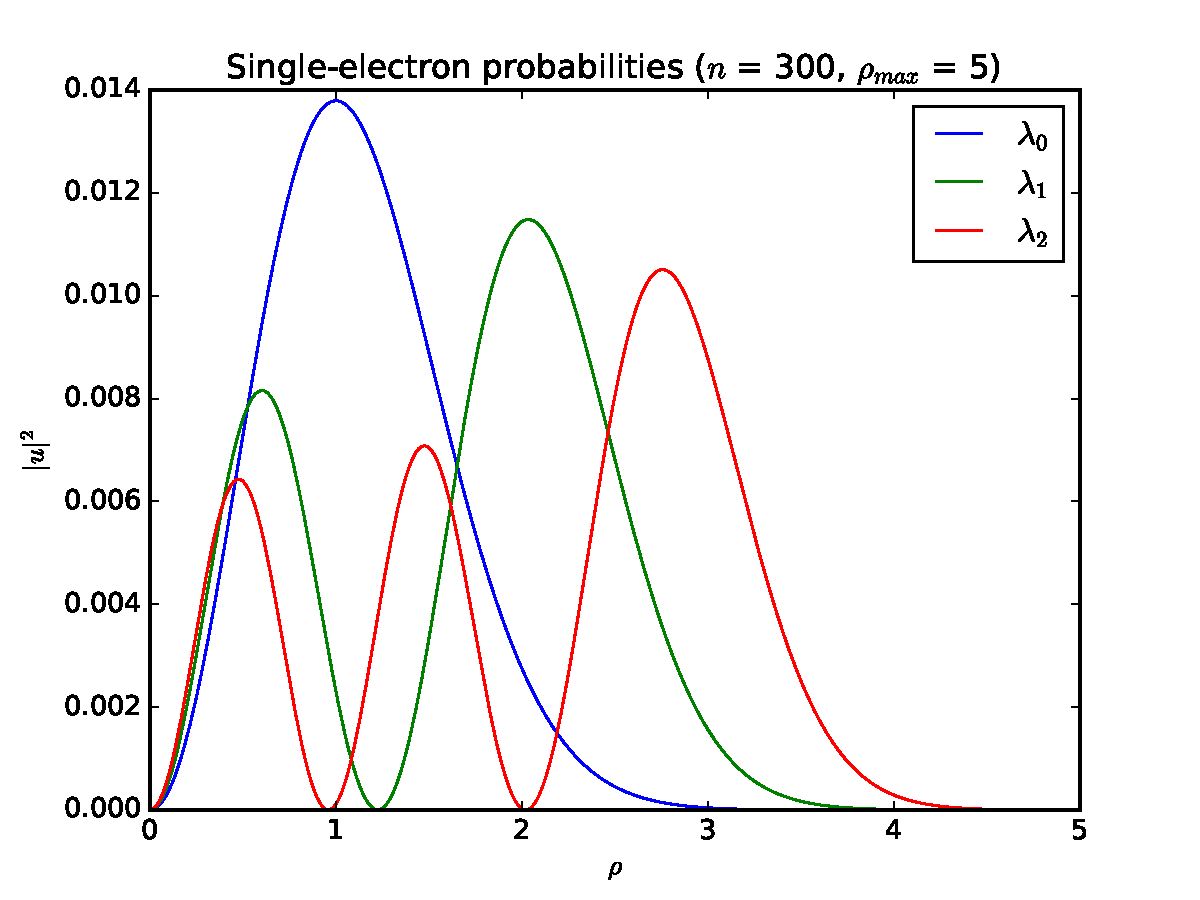
\includegraphics[width=\linewidth]{3_single_electron_probabilities_300.pdf}
	\caption{Probability distributions for the three lowest energy levels of an electron in an harmonic oscillator.}
	\label{fig:selprob300}
\end{figure}\\
A small eigenvalue corresponds to a low energy state for the electron. For lower energies, the electron is more likely to be closer to the origin. In addition, we see that the probability distribution gets more spread out at higher energies, and splits into multiple parts. So for instance for the $\lambda_2$ energy state there are three different radii that the electron is relatively likely to be found close to.

\FloatBarrier
\subsection{Two electrons} \label{section:twoe}
Figures \ref{fig:delprob} and \ref{fig:delprob2} show the probability distribution for different potential strengths $\omega_r$, for both the non-interacting and interacting case. They plot the same data, but the horizontal axis of the latter plot has been made logarithmic for clarity.\\
\begin{figure}[!h]
	\centering
	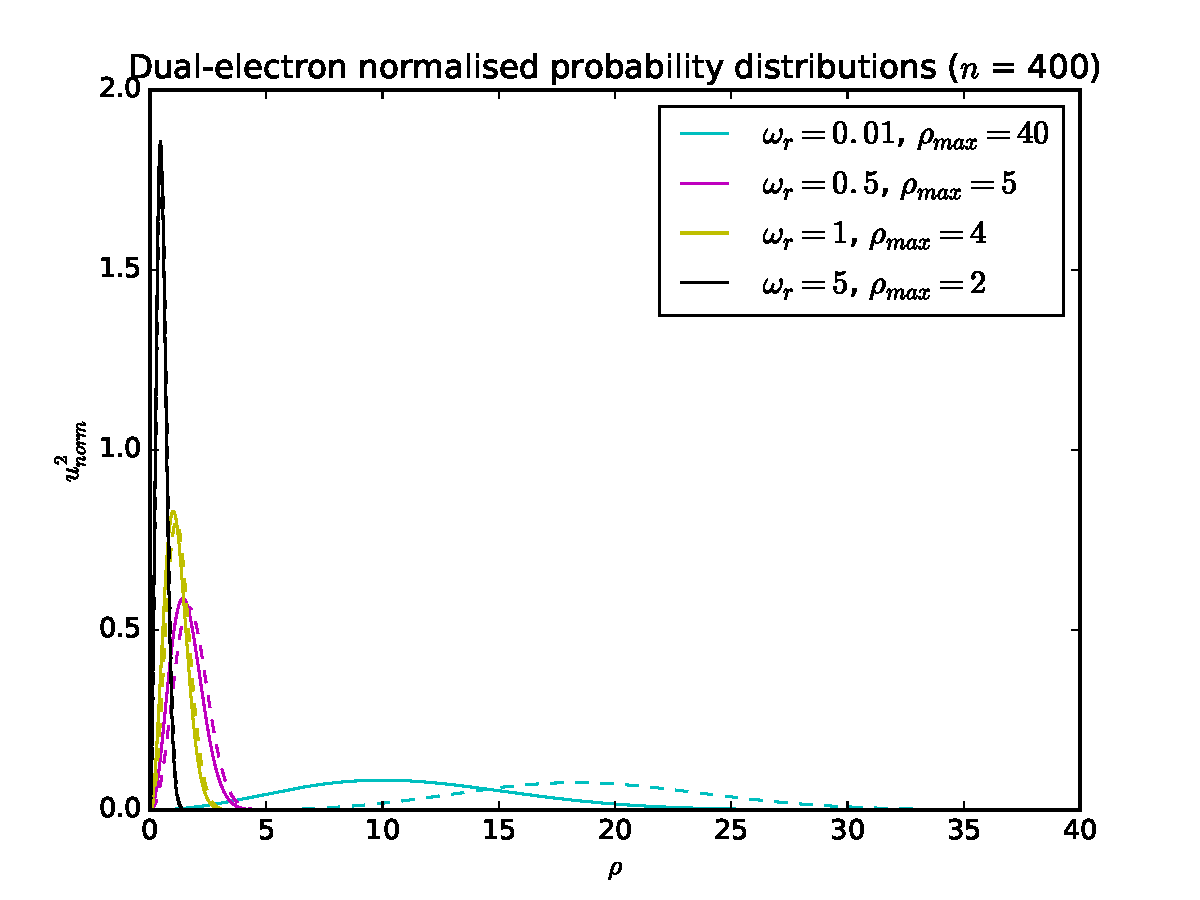
\includegraphics[width=\linewidth]{dual_electron_norm_probs.pdf}
	\caption{Normalised probability distributions for the ground state, for different values of $\omega_r$. The solid lines are for the non-interacting case, while the dashed lines are for the interacting case.}
	\label{fig:delprob}
\end{figure}
\begin{figure}[!h]
	\centering
	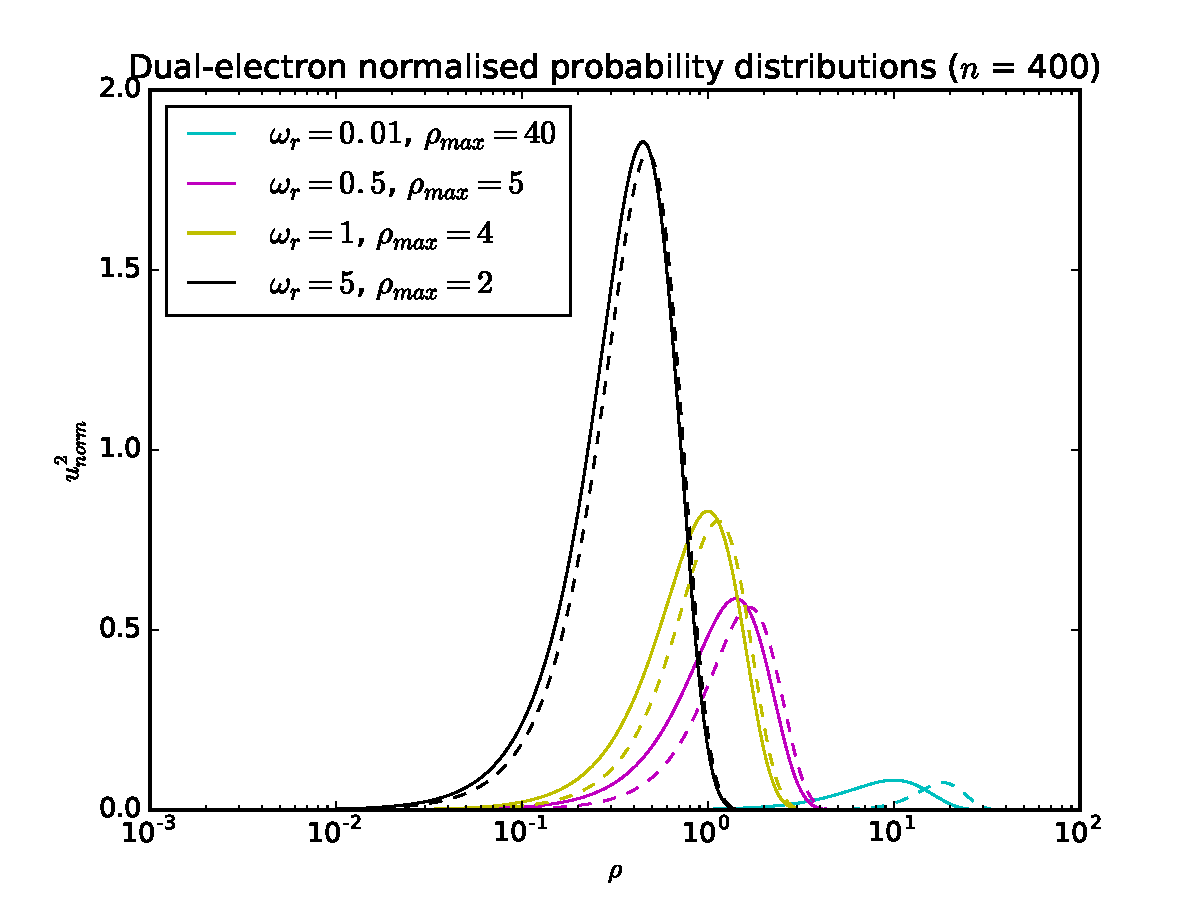
\includegraphics[width=\linewidth]{dual_electron_norm_probs2.pdf}
	\caption{Like figure \ref{fig:delprob}, only with logarithmic horizontal axis.}
	\label{fig:delprob2}
\end{figure}\\
These results are not quite surprising. Let us for a moment imagine that two electrons are bound together by a spring. The electrons oscillate back and forth due to the oscillation of the spring. They interact once when they are closest to each other (that is, the distance between them is the minimum).\\\\
For lower frequencies, the electrons will interact less frequently which means, by the analogy above, they are further apart from each other a lot more often. Another way to think of this is that the spring can be drawn over a larger distance before it is forced to contract, thus allowing the electrons to go further out. This can be seen from figure 1 (the blue line with $\omega_r = 0.01$) where the probability of them being close to each other is very small, while them being further apart is slightly larger.\\\\
For higher frequencies, the electrons will interact more frequently. Using the same analogy, we can think of the electrons bouncing back and forth very quickly. The spring is very stiff, so it cannot be stretched that far. Because of this, the electrons are forced to be very close to each other, which is exactly what we see in figure 1. In the case of $\omega_r = 5$ (the cyan line), we can clearly see that the probability of them being very close to each other is very large, while them being further apart is very low (practically zero).\\\\
Let us compare the interacting and non-interacting case. From figure \ref{fig:delprob2} we can see that the distance between the electrons are closer in the non-interactive case compared to the interactive case. The electrons will just oscillate back and forth when they are not affected by the Coulomb repulsion, and the max distance between the electrons are determined by the energy. In the interacting case however, the Coulomb repulsion causes the electrons to be pushed further apart. It serves as an extra pushing force between the electrons when they are close to each other.\\\\
Let us first think of a new analogy. We want to roll a ball upward a hill. In this case, the ball is the electron and the hill is the potential. If the hill is very steep (stronger potential), the distance the ball travels will be very short before it falls back down. On the other hand, if the hill is not very steep (weaker potential), the ball will be able to travel further away from us before it is forced to roll back. Figure \ref{fig:potil} shows an illustration of this.\\
\begin{figure}[!h]
	\centering
	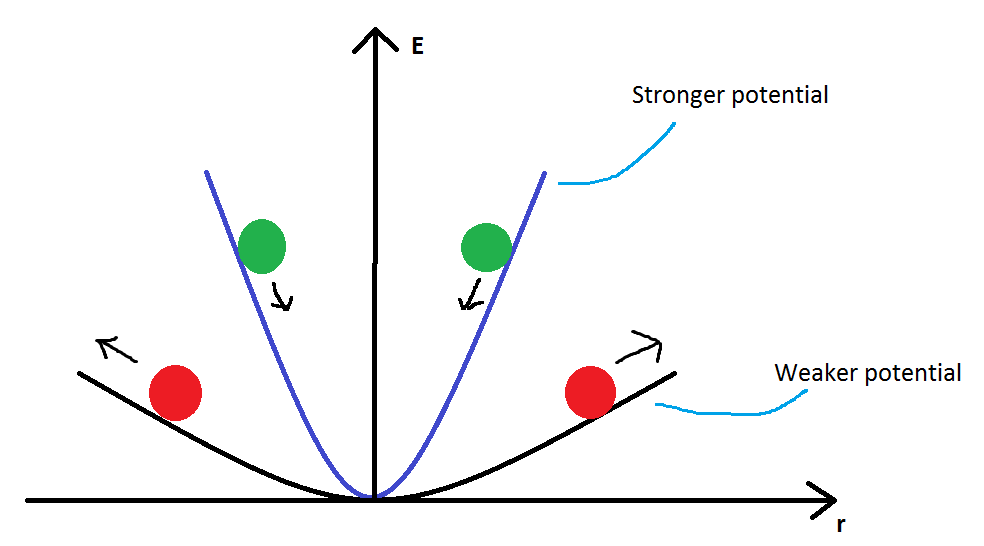
\includegraphics[width=\linewidth]{Potential_illustration2.png}
	\caption{An illustration of two different potentials and how they affect the electron.}
	\label{fig:potil}
\end{figure}\\
The probability distribution for the interacting and non-interacting case differ quite significantly for lower frequencies. The potential is not very steep for lower frequencies, so the electrons will not fall back down the potential as quick. With Coulomb repulsion, the electrons will be pushed further apart as the potential will not drag the electrons back fast enough.\\\\
With higher frequencies, the probability distributions will be very much alike. Higher frequencies gives a steeper potential, so the electrons will fall back down quicker because they are unable to climb the potential fast enough. Even with Coulomb repulsion, the electrons will not get very far due to the steep potential.\\\\
A different, but interesting, result can be seen in figure \ref{fig:tun}. What we can see here is the tunnelling effect. The red line shows the potential while the green line is the energy of the eigenvector. The energy and potential crosses each other at two points. What this means is that the distance of the electrons is bound between these two points and it cannot be anywhere outside them. However, the probability distribution says that the distance of the electrons can be smaller/larger than these two points. In classical mechanics, this would not be possible, but this is possible in quantum mechanics due to the tunnelling effect.\\
\begin{figure}[!h]
\centering
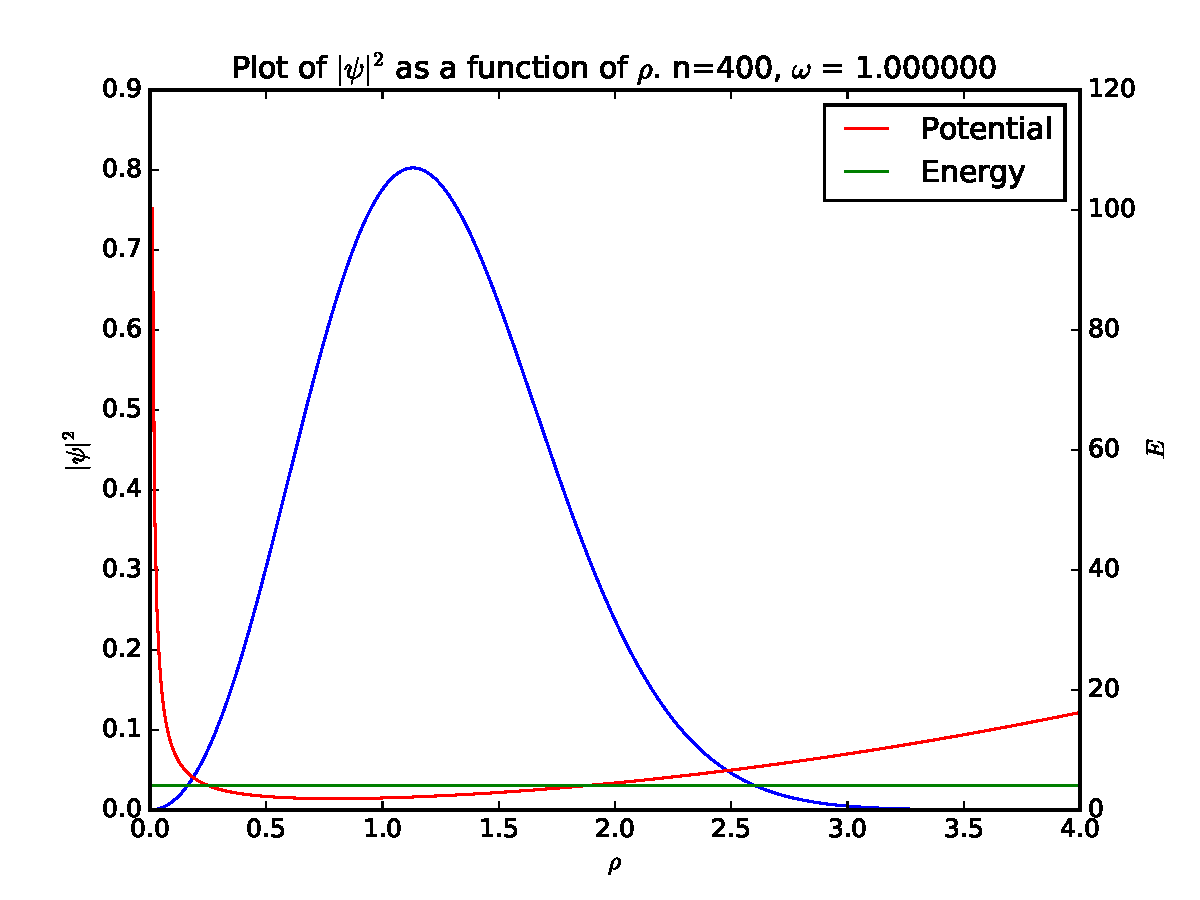
\includegraphics[width=\linewidth]{Plot_groundstate_tunneling_effect.pdf}
\caption{A plot showcasing the tunnelling effect. Plot for $\omega = 1$.}
	\label{fig:tun}
\end{figure}

\FloatBarrier
\subsection{Required number of iterations} \label{section:iters}
The number of similarity transformations required for reducing the matrix to diagonal form to a precision of $10^{-10}$ is plotted as a function of matrix extent in figure \ref{fig:iters}.\\
\begin{figure}[!h]
	\centering
	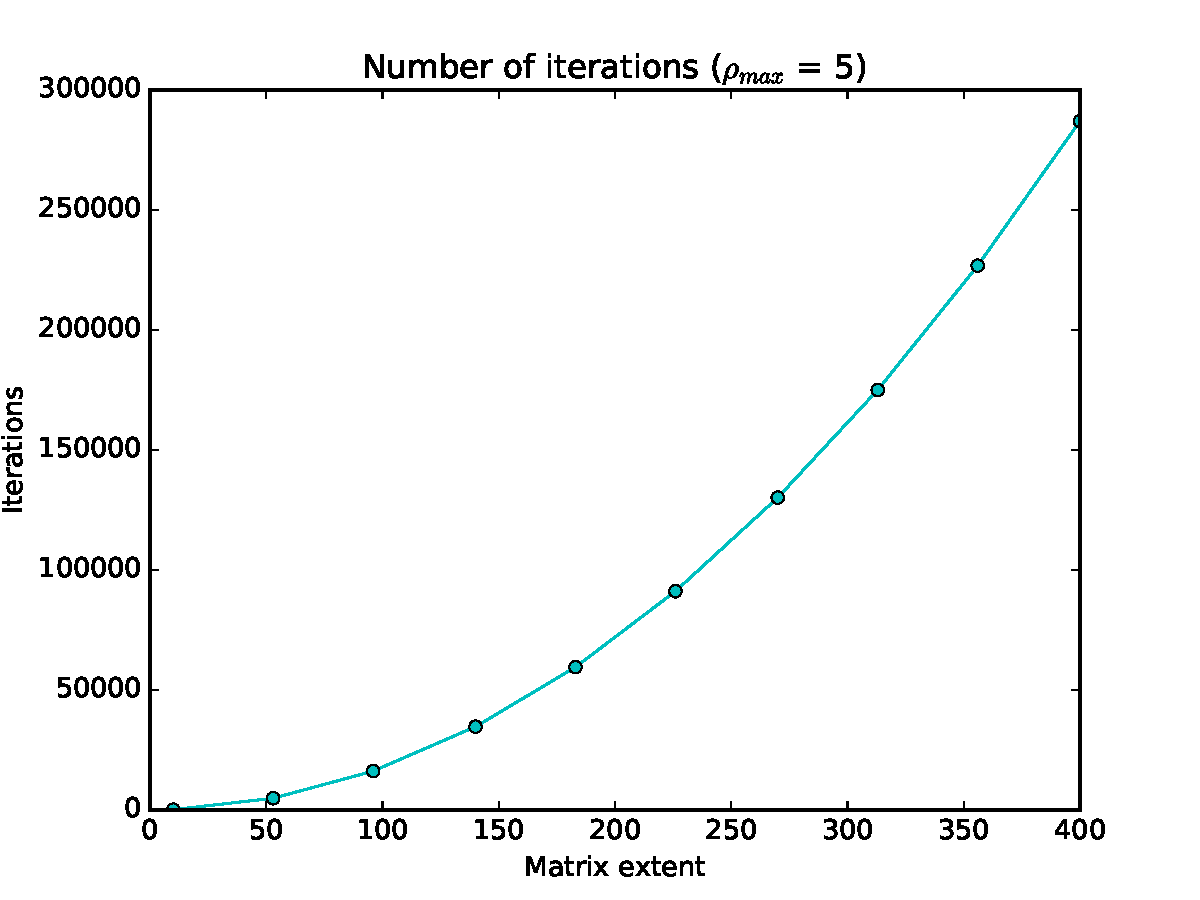
\includegraphics[width=\linewidth]{iterations.pdf}
	\caption{Number of Jacobi rotations as a function of matrix extent.}
	\label{fig:iters}
\end{figure}\\
By fitting this data with a polynomial (using Matlab), we found that the number of iterations go like $n^2$ (but also with a rather large coefficient in front of the $n$ term). From this we would expect the execution time to quadruple each time we double the extent of the matrix we are working on. This result seems reasonable from the algorithm, since it involves the elimination of at least $(n^2 - n)/2$ distinct off-diagonal elements (probably more, since previously eliminated elements won't necessarily stay eliminated).

\FloatBarrier
\section{Conclusions} \label{section:conc}
The run time of the Jacobi's method is quite slow, which implies that this algorithm is not exactly the smartest algorithm to use in order to solve eigenvalue problems. This is especially true if we compare Jacobi's method to other algorithms, e.g. the eig\_sym function of Armadillo, which finished in less than a second, compared to the 6 minutes in the C++ program.\\\\
Our eigenvalue results did not reach 4 decimal precision, but did come very close. One could possibly fix that by increasing the number of mesh points $n$ as well as $\rho_{max}$. However, as shown from the results, increasing $n$ would also increase the run time of the program, which is probably not practical for our purpose.\\\\
From the results, we saw that the average distance between the electrons will be larger when the harmonic oscillator potential is smaller (and vice versa for larger potentials). One can also see that the Coulomb repulsion will cause a larger effect for smaller potentials. 

\begin{thebibliography}{1}
	\bibitem{cpyhsics} M. Hjorth-Jensen, \emph{Computational Physics}, 2015, 551 pages
\end{thebibliography}

\end{document}
